\documentclass[english,a4paper,twocolumn,amsmath,amssymb,floatfix]{revtex4-1}
\usepackage[english]{babel}
%\renewcommand{\danishhyphenmins}{22}		%Giver mulighed for dansk orddeling. Slet kun hvis du VED hvad du laver, eller skal skrive noget på engelsk.
\usepackage[utf8]{inputenc}	%Hvis du benytter windows i stedet for linux, så skift utf8 ud med latin1. Tillader danske tegn.
\usepackage[T1]{fontenc}	%Tillader danske tegn
\usepackage{graphicx}		%Tillader indsættelse af billeder
\usepackage{dcolumn}		%Bruges til at lave matematiske tabelsøjler... se datatabel
\usepackage{booktabs}		%linjer i tabeller...
\usepackage{mathtools}		%Ekstra matematik... bare lad den være, du får muligvis brug for den.
\usepackage{siunitx}	%Bruges \SI{<tal>}{<enhed>}, \si{<enhed>} eller \num{<tal>}.
\usepackage{gensymb}
\sisetup{output-decimal-marker={,},separate-uncertainty=true}%Sørger for komma som decimalmarkør. Virker også ved decimaltal, hvis man bruger \num{<tal>}.
\usepackage{url}		 %bruges til at formattere url'er... kan sagtens udelades.
%Det følgende laver to makroer, \tref{} og \fref, der kan bruges ligesom \ref til at referere til hhv. tabeller og figurer. 
%De indsætter selv ordet Tabel/Figur, og sørger for at der ikke sker et linjebrud mellem dette og nummeret.
\newcommand{\tref}[1]{\tablename~\ref{#1}}
\newcommand{\fref}[1]{\figurename~\ref{#1}}
%Tilsvarende for ligninger. Indsætter "ligning (#)".
\newcommand{\lref}[1]{ligning~\eqref{#1}}
	% \eqref laver en reference med parenteser omkring (til brug ved ligninger.)
\newcommand{\picos}[0]{\textsc{PicoScope}} %hedder \picos for ikke at komme i kambolage med pico fra SIunits.
\newcommand{\epw}[0]{\textsc{EasyPlot}}    %epw er navnet på programfilen for easyplot, men det har ingen betydning for makroen. Jeg valgte det fordi det var noget jeg kunne huske, og det kan sagtens ændres.
\newcommand{\matl}[0]{\textsc{Matlab}} %Skriver Matlab med small caps.

%hyperref-pakken kan bruges til at redigere pdf-metadata. Det kan være et nice touch, men er generelt ikke påkrævet. Laver automatisk referencer i teksten til farvede hyperlinks i.
\usepackage{hyperref}
\hypersetup
{   pdfsubject={Rapport},
	pdfauthor={Anne Andersen}
    pdftitle={Røntgenøvelsen},
    pdfstartview=FitH,
    colorlinks=true}
    
%Følgende gør, at subscripts bliver ikke-kursiv. Anvendes X_|<subscript>|. Erstattes evt. med X_{\mathrm{<subscript>}}.
\makeatletter
\begingroup
\catcode`\_=\active
\protected\gdef_{\@ifnextchar|\subtextup\sb}
\endgroup
\def\subtextup|#1|{\sb{\textup{#1}}}
\AtBeginDocument{\catcode`\_=12 \mathcode`\_=32768 }
\makeatother

\usepackage[danish=quotes]{csquotes} %Danske citationstegn. \enquote{}

%Lad disse to linjer være. De sørger for at bunden af siden bliver pæn, og fjerner indryk ved afsnit.
\raggedbottom
\parindent = 0pt

\begin{document}

%Dette er boksen i toppen. Lad den være.
\framebox[\textwidth][l]{\textbf{
\begin{tabular}{p{\linewidth}l}
Received date:  & {Approved:}\\
& Date:\\
& Signature:\\
(reserved for instructor) & \\
\end{tabular}
}}
%Boksen slutter her.

\bigskip
\title{Experimental Physics III, Experiment 4: Rutherford scattering}

\author{Kirstine Juul} %Forfatter 1
 \altaffiliation{Department of Physics and Astronomy, Aarhus University, Denmark}
\author{Laurits Stokholm} %Forfatter 2
 \altaffiliation{Department of Physics and Astronomy, Aarhus University, Denmark} 
\author{Henriette Ravn} %Forfatter 2
 \altaffiliation{Department of Physics and Astronomy, Aarhus University, Denmark} %Hvis begge personer studerer det samme sted, kan informationen her flyttes til \affiliation
 \affiliation{Team number 1D} %Det er nok de færreste der er så priviligerede at have holdnummer pi, så skift denne tekst ud
	% Bemærk at det har betydning hvor \affilliation og \altaffiliation er placeret i forhold til \author. De virker på alle forfattere der kommer før dem.
\date{\today} %Dato. Husk at ændre!

\begin{abstract}
\bigskip
% his drug dependency vs. his denpendence on drugs
These experiments studies the Rutherford scattering of protons on atomic nuclei. Energetic 400 keV protons were generated using a Van de Graaff accelerator and directed onto thin metal foils of Au/C, LiF, B, and Al and the scattering cross section of the target atoms was measured as a function of the scattering angle in the range xx to 160 degrees. The cross section showed a clear angular dependency as ....., as expected. 
The thickness of the target layers Au/C were determined from the stopping power of the layers to be ..... The nuclear reactions of protons with boron were demonstrated by ... 
Mere is den dur bla bla bla ... 
In conclusion ... 
\end{abstract}

\maketitle

\noindent
\section*{Introduction}
The aim of this experiment was to use a particle accelerator to test certain dependencies of Rutherford scattering. Numerically, the Rutherford scattering differential cross section per target atom for any target atom is
\begin{equation}
\frac{d\sigma}{d\Omega} = 1.296 \left( \frac{Z_1 Z_2}{E_\infty [MeV] \, \sin^2 \left(\frac{\theta}{2} \right) }\right)^2\left[\frac{mb}{sr}\right],
\end{equation}
where $\theta$ is the scattering angle, $Z_1$  is the atomic number of the incident particles, $Z_2$ is the atomic number of the target nuclei, and $E_{\infty}$ is their kinetic energy HUSK CITE!%cite 
. 
In order to test these dependencies a relation between the cross section and the count rate (number of scattered particles per time) is found as
\begin{equation}
dN = N \, n_{\text{tar}} \, dx \,d\Omega \, \frac{d\sigma(\theta,\phi)}{d\Omega},
\end{equation}
where $N$ is the number of incoming particles per time, $n_\text{tar}$ is the particle density of the target, $dx$ is the thickness of the target, and $d\Omega$ is the solid angle of the detector.




\section*{Materials and Methods}

\subsection*{Experimental setup}
The energetic incident protons were generated using a Van de Graff accelerator. The accelerator ionized a hydrogen gas which could escape in a narrow beam. The particles were accelerated to an energy up to 400 keV controllable on the accelerator. The particles entered a big electromagnet which makes a magnetic field that controls the angle of deflection of proton beam. By adjusting the field one could control which particles, depending on the mass and charge, could enter the beamline. 

%\begin{figure}
%OBS:
%Hvis man bruger TeXnicCenter under windows til editering af TeX filer,
%kan man ikke inkludere .eps grafik filer ved konvertering til .pdf.
%Man kan i stedet anvende f.eks. .jpg eller .png filer
%\centering
%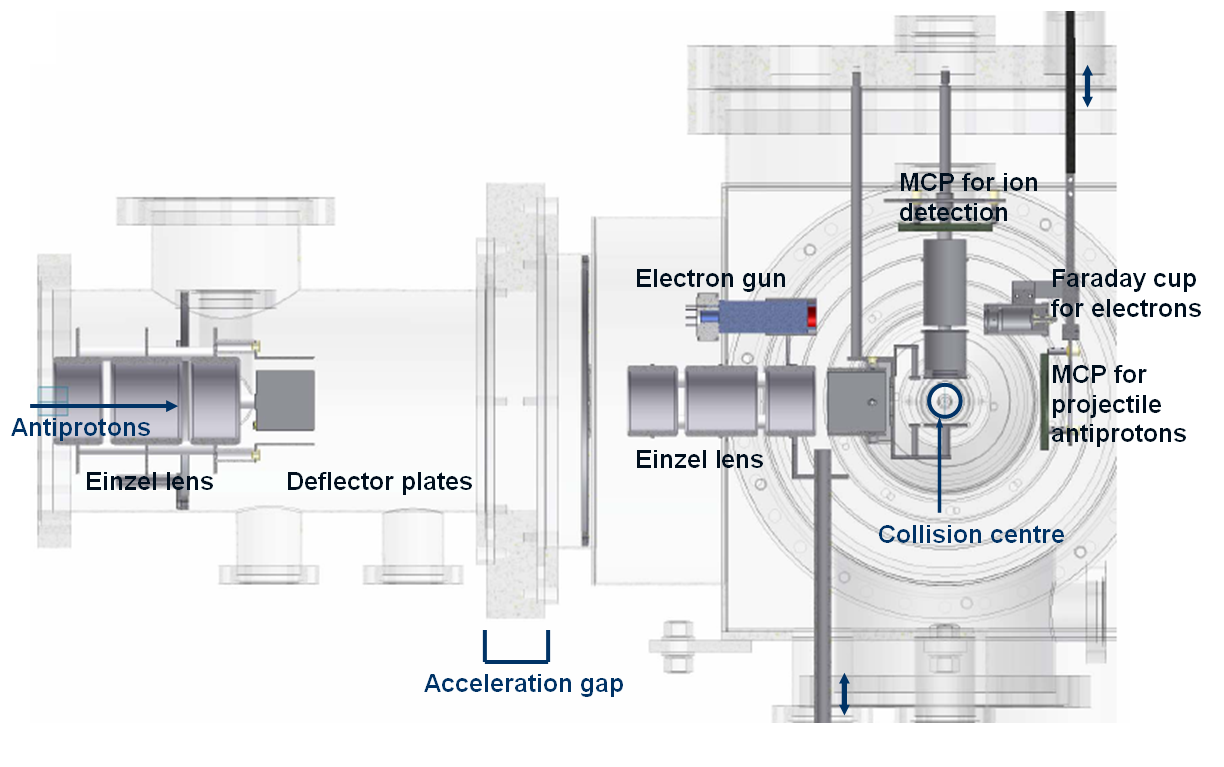
\includegraphics[width=0.9\columnwidth]{figure1.png}
%\caption{\sl Opstilling til første del af øvelsen. Her ses....}
%\label{fig:en_label} %Bruges til referencer. Husk at den SKAL stå efter den tilhørende "\caption{}"
%\end{figure} 

From the beamline the particles were directed toward a chosen target material, where they got scattered on atomic nuclei of the target. A detector was placed at a movable position around the target, such that scattering angles up 160 degrees could be measured. 
The detector was coupled to a digitizer with a time resolution of xx s and  connected to a computer. During measurements the digitizer started a clock inside it. When the detector was hit by a particle, the digitizer translated the measured energy into a digital number and sent the number and the corresponding time stamp to the computer. 
The program Mc2Analyzer was used to handle the data. The digital number is an arbitrary number called a channel number. It is translatable to the actual energy by a linear factor plus an offset. In order to convert these channel numbers to correct energies of the scattered particles a calibration was done.


\subsection*{Calibration}
The measured energy of a scattered particle is given as a digital output called a channel number. A calibration is necessary to convert these channel numbers to the actual particle scattering energies. Assuming a linear relationship between the energy and the channel number the energy can be found as 
\begin{equation}
E = \alpha(k - k_0),
\end{equation}
where $k$ is the channel and $k_0$ and $\alpha$ are constants. The constants in the relation is determined by varying the incoming energy and writing down the corresponding values of energy and channel number. The constants are determined from a linear fit of the energies as function of channel numbers.
With the Van de Graff accelerator the magnetic field can be adjusted to deflect either $\mathrm{H^+}$ or $\mathrm{{H_2}^+}$ into the beamline. For each of these a data point of energy related to channel number can be found. 
By considering energy and momentum conservation for elastic scattering in two dimensions the energy of the scattered particles $E_f$ can be found from the incident proton energy and the scattering angle as: 
\begin{equation}
E_f = \left( \frac{m_p \cos\theta + \sqrt{{m_t}^2 - {m_p}^2 \sin^2\theta}}{m_p+m_t} \right)^2 E_i,
\end{equation}
where $E_i$ is the energy of the incident beam particles, $m_p$ and $m_t$ are the masses of the incident protons and the target particles, respectively, and $\theta$ is the angle between the direct outgoing non-scattered beam and the scattered particles - also called the scattering angle.

Unfortunately, this only give two data points one from $\mathrm{H^+}$ and one from $\mathrm{{H_2}^+}$. The incline from the linear fit to these data points is still useful. However, another method is used to determine the zero-amplitude constant $k_0$. Different energies are generated using a pulse generator by changing the amplitude (corresponding to a change of resistance). For each fixed amplitude, a normal distribution of counts around a certain mean channel is obtained. The mean channel (also called the centroid) is determined from a Gaussian fit to the distribution. 

TABLE WITH CORRESPONDING VALUES OF AMPLITUDE AND MEAN CHANNEL (AND THEIR UNCERTAINTIES)!

FIGURE WITH AN EXAMPLE OF A GAUSSIAN FIT.

Figure X shows the count distribution as function of channels for the amplitude X fitted with gaussian function. The data clearly follows a gaussian distribution and the data points are, within uncertainty, well described by a gauusian distribution. 

From the fit the coefficient $k_0$ is .... \\



\subsection*{Targets}
Something about the different targets... Rettes til når vi ved noget mere.

The targets and their corresponding thickness and areal density are noted in Table ...

\begin{table}[h]
\centering
\caption{\sl De målte data for kalibreringen af....}\begin{tabular}{l D{.}{,}{5.0} *{2}{ D{.}{,}{10.0} @{$\pm$} D{.}{,}{2.0} } D{.}{,}{3.0}}
\toprule
 \multicolumn{1}{c}{Target} & \multicolumn{2}{c}{Thickness (Å)} & \multicolumn{2}{c}{Area density} \\
\midrule
LiF/C  &  ?  &  ? & 0.5 \\
B/C  &  ?  &  ?  \\
AL  &  ?  &  ?  \\
Au/C  &  ?  &  ?  \\
\bottomrule
\end{tabular}
\label{tbl:eksempel}
\end{table}




\section*{Angular dependency of the Rutherford cross section}

\section*{Angular dependency of the proton energy}

\section*{Target dependency of the Rutherford cross section}

\section*{Thickness of the target layers} 

\section*{Nuclear reactions of protons with boron}

\begin{table}[h]
%I denne tabel bruger jeg søjletypen D{#1}{#2}{#3} fra pakken dcolumn. Denne sætter hele søjlen i matematik-mode, og justerer
%indholdet, således at #1 bliver justeret over hinanden. I det færdige output bliver #1 erstattet med #2. og i #3 angiver man antallet af 
%tegn før og efter #1 (syntax: før.efter).
%\multicolumn{#4}{#5}{#6} tillader at forhindre matematikmode i en række. #4 giver antallet af søjler der skal kombineres, her 1 eller 2, #5 giver den søjlejustering der skal gælde, her c, og #6 giver det der skal stå i feltet.
% koden @{$\pm$} udskifter et søjlemellemrum med et plus-minus tegn, således at data angives i en søjle og usikkerhederne i den næste. Generelt udskifter @{#7} søjlemellemrum ud med #7.
% *{#8}{#9} bruges til at gentage #9 det antal gange som #8 angiver, her 2.
\centering
\caption{\sl De målte data for kalibreringen af....}%Tabelforklaringer placeres normalt over tabellen.
\begin{tabular}{l D{.}{,}{1.2} *{2}{ D{.}{,}{1.2} @{$\pm$} D{.}{,}{1.2} } D{.}{,}{1.3}}
\toprule
  & \multicolumn{1}{c}{E (\si{\mega\electronvolt})} & \multicolumn{2}{c}{I (\si{\ampere})} & \multicolumn{2}{c}{V (\si{\milli\volt})} & \multicolumn{1}{c}{K (\si{\centi\meter})} \\
\midrule
aaaa  &  3.44  &  1.23 & 0.03  &  3.67 & 0.04  &  0.012 \\
bbbb  &  2.44  &  1.45 & 0.05  &  2.89 & 0.02  &  0.023 \\
cccc  &  1.44  &  2.67 & 0.02  &  3.99 & 0.07  &  0.089 \\
\bottomrule
\end{tabular}
\label{tbl:eksempel}
\end{table}


%\begin{figure*} %Det er stjernen der gør forskellen. Husk at den også skal være i \end.
%	\centering
%	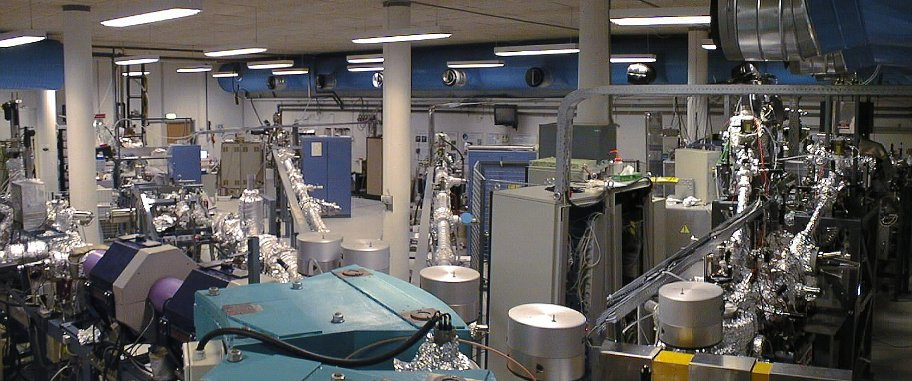
\includegraphics[width=\textwidth]{figure2.jpg}
%	\caption{\sl Benyt denne kommando hvis du skal indsætte en figur som er for bred til at kunne være i en enkelt kolonne. Virker tilsvarende for tabeller.}
%\end{figure*} 


\section*{Discussion}

%\begin{figure}
%	\centering
%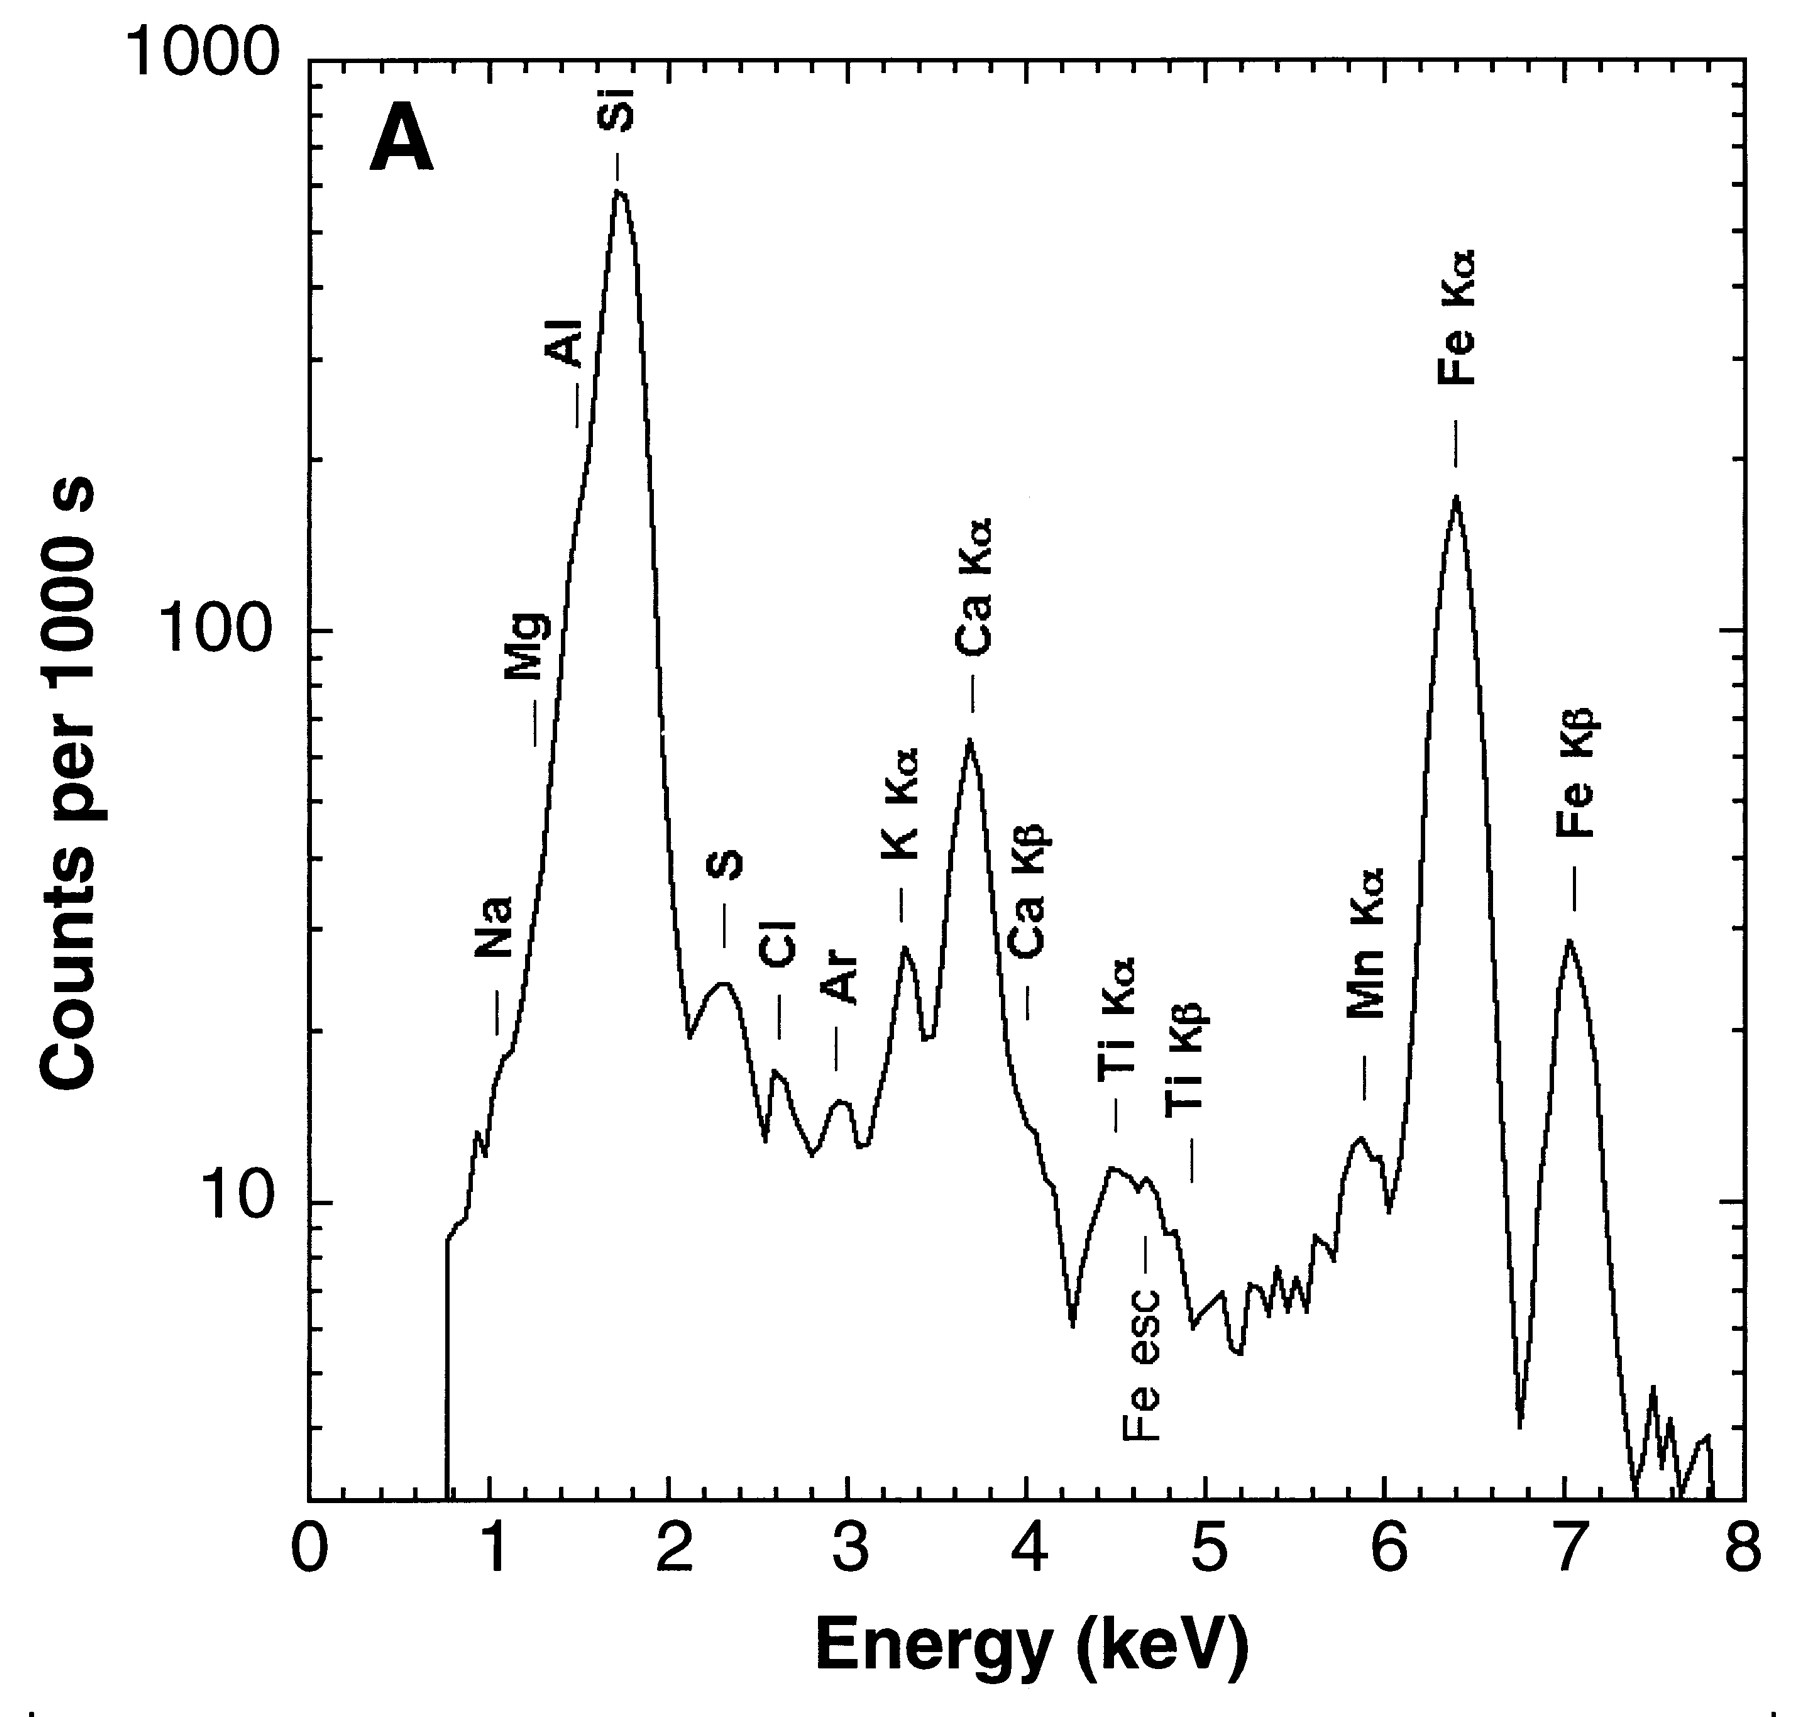
\includegraphics[width=0.9\columnwidth]{figure3.jpg}
%\caption{Energikalibrering}
%\label{fig:kalibrering}
%\end{figure}

\section*{Conclusion}

\appendix
\section*{Bemærkninger}
\textsl{ Denne template (skabelon) er ment som en rettesnor for rapportens indhold og udseende. De enkelte afsnit og deres rækkefølge skal selvfølgelig tilpasses den enkelte øvelse. Det er derimod vigtigt at du holder dig til layout (skrifttyper, marginer, kolonner,...), som en øvelse i at skrive rapporter og artikler hvor designet ofte er forudbestemt. Af hensyn til rettelses-proceduren bedes du beholde \enquote{kassen} over overskriften. Denne \LaTeX-template bygger på REVTeX 4.1--pakken fra The American Physical Society, og er blevet tilpasset af Peter Birk Nielsen (mindre revision 2013 af Jonas Refsgaard). For mere info om \LaTeX{}, se Daleif \cite{Daleif}}

\begin{thebibliography}{99}
\section*{REFERENCES}

\bibitem{hk:1}
Eksperimentelle øvelser i fysik, øvelsesvejledninger efteråret 2006, IFA, Aarhus Universitet
\bibitem{hk:2}
	Se: \url{www.inkscape.com}
\bibitem{Daleif}
	Dalifs bog om \LaTeX. \url{http://www.imf.au.dk/system/latex/bog/version3beta.html}

\end{thebibliography}

\end{document}

